% Need these new commands to compile:
%\newcommand{\todo}[2]{\textcolor{red}{\textbf{TODO (#1): #2}}}
%\newcommand{\comment}[1]{\textcolor{blue}{\textbf{#1}}}



\section{Strong Lensing}
\textit{ Authors: Simon Huber\footnote{shuber@mpa-garching.mpg.de}, Sherry H.~Suyu\footnote{suyu@mpa-garching.mpg.de}, Tanja Petrusevska\footnote{tanja.petrushevska@ung.si} }

The Hubble constant $H_0$ is one of the key parameters to describe the
universe. Current observations of the CMB (cosmic microwave
background) assuming a flat $\Lambda$CDM cosmology and the standard
model of particle physics yield $H_0 = \SI[separate-uncertainty =
true]{67.36 \pm 0.54}{\kilo\meter\per\s\per\mega\parsec}$
\citep{Planck:2018vks} which is in tension with $H_0 =
\SI[separate-uncertainty = true]{73.52 \pm
  1.62}{\kilo\meter\per\s\per\mega\parsec}$ from the local distance ladder
\citep{Riess:2016jrr,Riess:2018byc}. In order to verify or refute this
$3.6 \sigma$ tension, further independent methods are needed. 

One such method is lensing time delay cosmography which can determine
$H_0$ in a single step. The basic idea is to measure the time delays
between multiple images of a strongly lensed variable source
\citep{Refsdal:1964}. This time delay, in combination with mass
profile reconstruction of the lens and line-of-sight mass structure,
yields directly a ``time-delay distance'' that is inversely
proportional to the Hubble constant ($t \propto D \propto
H_0^{-1}$). Applying this method to four lensed quasar systems, the
H0LiCOW collaboration \citep{Suyu:2016qxx} together with the
COSMOGRAIL collaboration
\citep[e.g.]{Eigenbrod:2005ie,2013Tewes,2017Courbin} measured $H_0 =
72.5^{+2.1}_{-2.3} \, \si{\kilo\meter\per\s\per\mega\parsec}$ in flat
$\Lambda$CDM \citep{Birrer:2018vtm}, which is in agreement with the
local distance ladder and higher than CMB measurements.  Another
promising approach goes back to the initial idea of
\cite{Refsdal:1964} using lensed supernovae (LSNe) instead of quasars
for time-delay cosmography. Here we investigate the prospects of using
LSST for measuring time delays of both lensed supernovae and lensed
quasars.

\subsection{Supernovae Lensed by Galaxies}
\textit{Contributors: Simon Huber, Sherry H.~Suyu}

Even though the number of LSNe is significantly lower than the number of
lensed quasars, LSNe have some important advantages. First 
the sharp rise
and decline of SN light curves make time-delay measurements easier and possible
on shorter time scales in comparison to stochastically varying quasars. Second LSNe Ia are very promising
to break the model degeneracies \citep{Schneider:2013wga} in two
independent ways using dynamics \citep{Barnabe2011,2017:Yildirim} or
the standard candle nature of SNe Ia.  

So far only two systems with resolved
multiple images have been observed, namely SN ``Refsdal''
\citep{Kelly:2015xvu,Kelly:2015vjq} and iPTF16geu
\citep{Goobar:2016uuf}. But LSST will play a key role to detect many
more LSNe. At the moment we expect to find approximately $50$ resolved
LSNe Ia \citep{Oguri:2010} or $900$ in total \citep{Goldstein:2017bny}
over the 10 year survey. No other survey is capable of providing such
high numbers.

The goal of this section is to evaluate different
cadences for LSNe time-delay measurements. For this purpose we have investigated
14 different observing strategies: 11 from the call for whitepapers
(baseline2018a, kraken\_2026, colossus\_2665, pontus\_2002,
colossus\_2664, colossus\_2667, pontus\_2489, kraken\_2035,
mothra\_2045, pontus\_2502,
kraken\_2036)\footnote{\url{http://astro-lsst-01.astro.washington.edu:8080/}},
pontus\_2506 which is a cadence from Tiago Ribeiro doing the revisit
after 30 minutes in different filters, and alt\_sched and
alt\_sched\_rolling from Daniel Rothchild and collaborators
\footnote{\url{http://altsched.rothchild.me:8080/}}. In the future, we
will also investigate the new cadences kraken\_2042, kraken\_2044,
mothra\_2049 and nexus\_2097. To simulate observations randomly, we have used 202
mock LSNe Ia from the OM 10 catalog \citep{Oguri:2010},
and produced the light curves for the mock SNe images with
the spherically symmetric SN Ia W7 model \citep{1984:Nomoto}
calculated with ARTIS (Applied Radiative Transfer In Supernovae)
\citep{Kromer:2009ce} in combination with magnifications maps from
GERLUMPH \citep{Vernardos:2015wta} to include the effect of
microlensing similar as in \citep{Goldstein:2017bny}. We then simulate
data points for the light curves, following the observation pattern from different cadences
and uncertainties according to the LSST science book
\citep{2009:LSSTscience}. To measure the time delay from the simulated
observation we use the free knot spline optimizer from PyCS (Python
Curve Shifting) \citep{2013:Tewesb,Bonvin:2015jia}. Details of this
work will be presented in Huber et al. (in preparation).


The structure of this subsection is organized as follows. In
\ref{sec:simulation of mock data} we describe how we simulate and
evaluate the mock data and in \ref{sec:results} we present our results
where we have quantified 14 cadences for LSNe Ia.

\subsubsection{Simulating and evaluating mock data}
\label{sec:simulation of mock data}
To simulate mock data for the different cadences we have picked 10
fields in the WFD (wide fast deep survey) which are listed in Table
\ref{tab: 10 wfd fields}. For a given cadence for each of these
fields, we store the following for each visit of the field: date
(mjd), filter(s) observed, and 5-$\sigma$ depth $m_5$. Such an
observing sequence of visits is illustrated for the ``baseline2018a''
cadence in figure \ref{fig:observation patter LSST 10 year survey},
where for one field in the WFD all observations within the 10 year
survey are shown. 
%
\begin{figure}
\centering
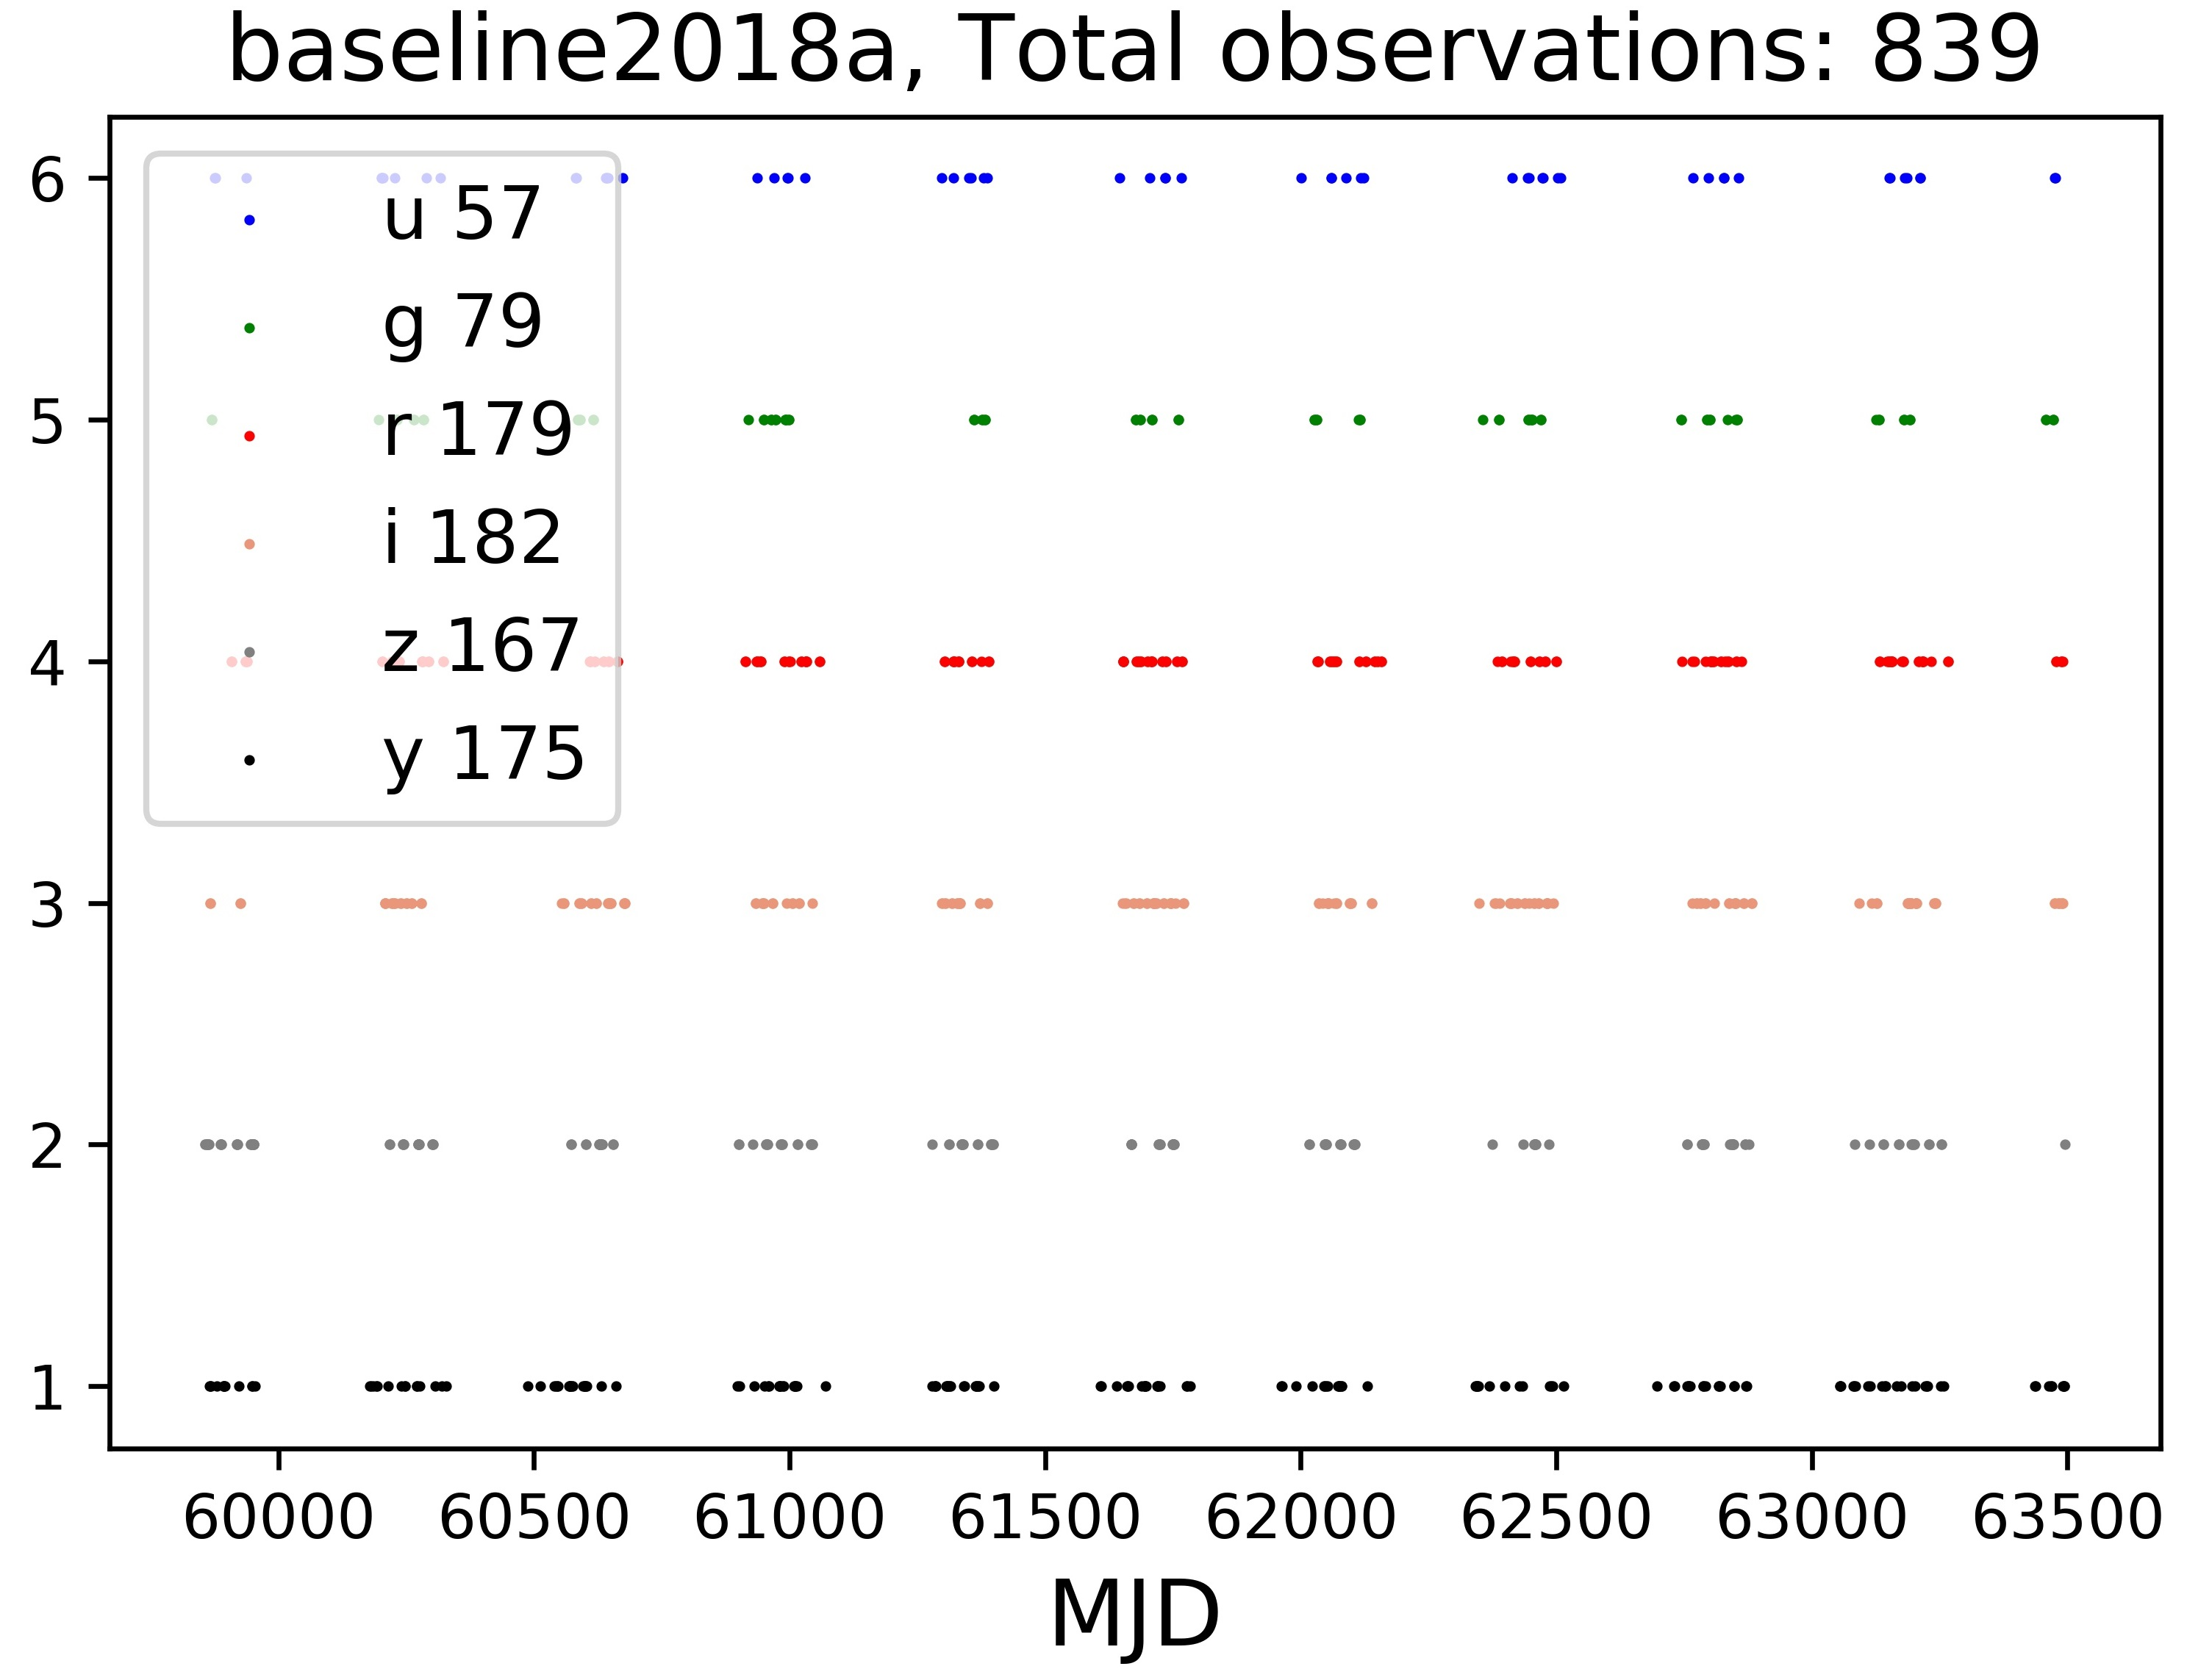
\includegraphics[scale=0.7]{figures/field_number3_baseline2018a_Daniel.jpg}
\caption{This illustrates for the observing strategy "baseline2018a" the mjd and filter when observations are taken over the 10 year survey for field number 4 in table \ref{tab: 10 wfd fields} in the wide fast deep survey}
\label{fig:observation patter LSST 10 year survey}
\end{figure}
%
\FloatBarrier 
To simulate observational data of a LSN system, we place randomly in
one of the 10 choosen fields from Table \ref{tab: 10 wfd fields} a
mock LSNe Ia from the OM 10 catalog, which is a mock catalog for
strong gravitational lenses \citep{Oguri:2010}. The catalog contains
about 400 LSNe Ia (The catalog is 10 times oversampled which means
that the total number of LSNe Ia is about 40) for LSST with an image
separation larger than $\SI{0.5}{\arcsec}$. For the lens model an SIE
(singular isothermal ellipsoid) \citep{Kormann:1994} is assumed and
therefore the time delay $\tau$, the convergence $\kappa$ and the
shear $\gamma$ is known for each of the multiple SNe images. By
assuming a W7 model and placing each of the SNe images randomly in the
corresponding magnification map one can calculate mock light
curves. Furthermore we place the mock system randomly in time, such
that the detection criterion applied in OM 10 is fulfilled. The
criterion is that the peak of the i-band magnitude of the fainter image
for a double or the 3rd brightest image for a quad, falls in the
observing season.
By combining this with the observing sequence, we get simulated
observations as illustrated in figure \ref{fig: simulated observation}
for a quad system. The error is calculated according to \cite[sec 3.5,
p. 67]{2009:LSSTscience}.
\begin{figure}[h!]
\centering
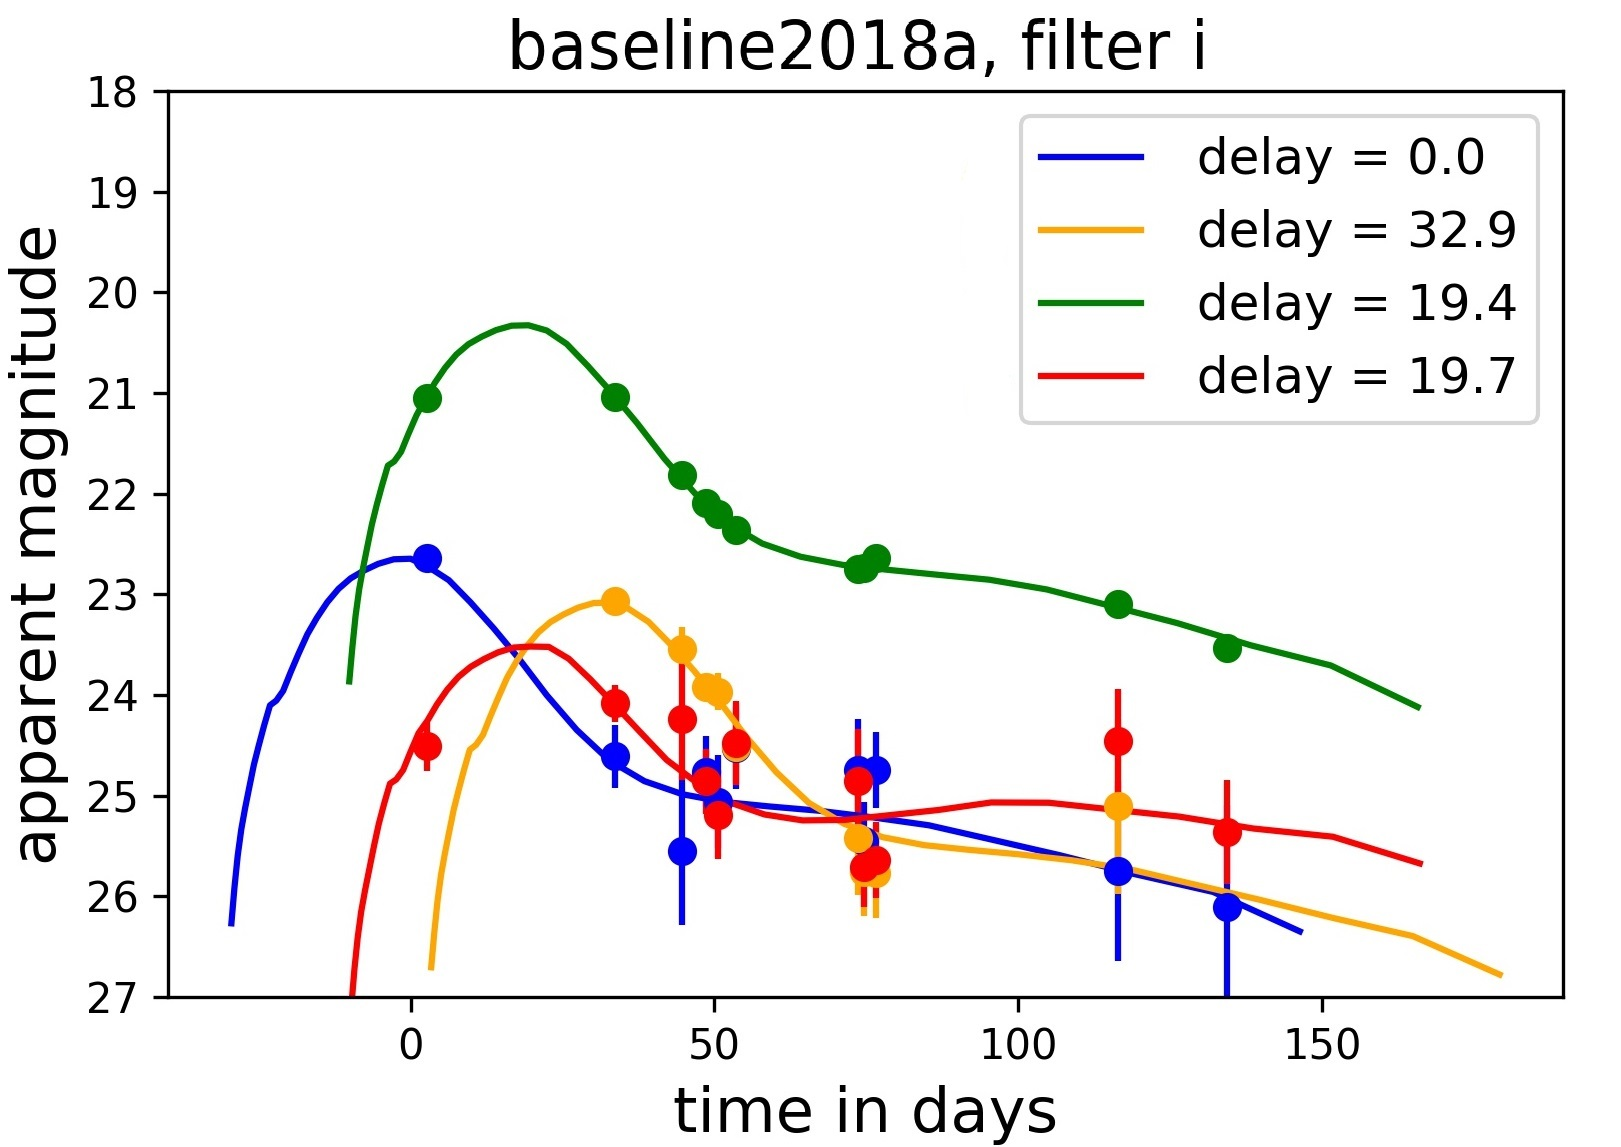
\includegraphics[scale=0.7]{figures/Obsevation_number399_baseline2018a_filter_i_oversampling_00.jpg}
\caption[]{In this figure the i-band light curves of a mock quad LSNe Ia are shown. The observation sequence is for a random field in WFD survey for the cadence "baseline2018a".}
\label{fig: simulated observation}
\end{figure}
%
\begin{table}
\centering
\begin{tabular}{c|c|c|c|c|c|c|c|c|c|c}
field number & 1 & 2 & 3 & 4 & 5& 6 & 7 & 8 & 9 & 10  \\
\hline
RA& 0.0 & 32.1 & 65.8 & 50.9 &44.9& 125.6 & 155.0 & 207.7 & 304.3 & 327.5  \\
\hline
DEC& -7.4 & -44.2 & -7.2 & -30.0 & -50.9& -11.4 & -25.6 & -45.3 & -55.2 & -35.9  \\
\end{tabular}
\caption{The 10 fields of the wide fast deep survey, where the observation sequence for different cadences was considered.}
\label{tab: 10 wfd fields}
\end{table}
%
\FloatBarrier

To evaluate the mock data and get a measured time delay we use the
free knot spline optimizer from PyCS (Python Curve Shifting)
\citep{2013:Tewesb,Bonvin:2015jia}. PyCS was initially developed to
measure time delays in strongly lensed quasars, and is not yet
optimised for LSNe Ia, such fitting simultaneously multiple filters
and using SN template light curves.  Applying PyCS to individual
filter's light curves, we get a single independent time delay for each
filter.  We combine the 6 delays from the 6 LSST filters afterwards
into a single delay, but we expect more precise and accurate delays by
using multi-color fitting in the future. We also expect improvements
in delay measurements with the use of SNe Ia template instead of
splines.  

%so there are still
%some improvements for LSNe Ia, which will be implemented in the
%future. The first one is that to date multi-color time delay fitting
%is not possible, which means that we get a single independent time
%delay for each filter. We combine this 6 delays afterwards to a single
%delay, but we expect more precise and accurate delays by using
%multi-color fitting. A second improvement might be the use of SNe Ia
%templates instead of splines. This means that we do a conservative
%time delay estimate and with future improvements we might be able to
%measure time delays even better. 

To have sufficient statistics, we investigate for each cadence
strategy 202 mock LSNe Ia, where we pick 50 \% doubles and 50 \%
quads. For each of the mock systems we draw 100 random starting
configurations. A starting configuration corresponds to a random
position in the microlensing map and a random field from Table
\ref{tab: 10 wfd fields}, where it is placed randomly in one of the
observing seasons such that the detection requirement from OM 10 is
fulfilled. For each of these starting configurations we then draw 1000
different noise realizations of light curves, where we also shift the
time delays for each noise realizations randomly by $-3$ to
$\SI{3}{\day}$, to estimate uncertainties of delay measurements with
PyCS. For each realization we calculate the deviation from the true
time delay as
%
\begin{equation}
\tau_\mathrm{d} = \frac{t_\mathrm{measured} - t_\mathrm{true}}{t_\mathrm{true}}.
\label{eq: deviation from true time delay}
\end{equation}
For one strategy and double LSNe Ia, we have thus $1 {\rm (delay for the
one pair of images)} \times 6 {\rm (filters)} \times 100 {\rm
(starting configurations)} \times 1000 {\rm (noise realisations)}$
time-delay deviations as in \eqref{eq: deviation from true time delay}.
%, where the 6 stands for the 6 LSST filters. 
For the 6 pairs of images for a quad system we have a sample of $6
\times 6 \times 100 \times 1000$. The resulting distribution of
time-delay deviation is investigated for each pair of images and each
filter separately. From the $100 \times 1000$ time-delay deviations we
define accuracy as the median $\tau_\mathrm{d,50}$ and precision as
$\delta = (\tau_\mathrm{d,84}-\tau_\mathrm{d,16})/2$, where
$\tau_\mathrm{d,84}$ is the 84th and $\tau_\mathrm{d,16}$ the 16th
percentile. Measuring $H_0$ with 1\% accuracy requires that the accuracy
in the delay deviation $\tau_\mathrm{d,50}$ is $<1\%$ (since $H_0 \propto
t_{\rm true}^{-1}$). Since the 6 time-delay deviations from the 6 filters are independent we combine them into a single time-delay deviation via the weighted mean. This means that in the end we have for one strategy and a mock LSNe Ia one 
\begin{equation}
\tau_\mathrm{d,50} \pm \delta
\label{eq: accuracy and precission}
\end{equation}
per pair of images.


\subsubsection{Results}
\label{sec:results}
In this section we summarize the results and quantify the 14
investigated cadences. Given that $H_0 \propto \frac{1}{t}$, where $t$
is the time delay between two images, we aim for accuracy
($\tau_\mathrm{d,50}$) smaller than 1 percent and precision ($\delta$)
smaller than 5 percent in equation \ref{eq: accuracy and precission},
and Table \ref{tab: fraction of systems} shows the fraction of systems
of the 202 mock lenses fulfilling that requirement. The accuracy
requirement is needed for measuring $H_0$ with 1\% uncertainty, and
the precision requirement ensures that the delay uncertainty does not
dominate the overall uncertainty on $H_0$ given typical mass modeling
uncertainties of $\sim 5\%$ \citep[e.g.,][]{Suyu2018}.  A quad system is counted as successful if one of the 6 delays fulfills this requirement.\\
%
\begin{table}
\centering
\begin{tabular}{c|c|c|c}
&total& doubles & quads \\
\hline
alt\_sched\_rolling & 13.9 \% & 10.4 \% &3.5 \% \\
\hline
alt\_sched & 10.4 \% & 8.4 \% & 2.0 \% \\
\hline
pontus\_2506 & 6.9 \% & 5.4 \% &1.5 \% \\
\hline
colossus\_2667 & 6.9 \% & 5.4 \% &1.5 \% \\
\hline
pontus\_2489 & 6.0 \% & 5.0 \% &1.0 \% \\
\hline
mothra\_2045 & 5.0 \% & 4.0 \% &1.0 \% \\
\hline
kraken\_2036 & 4.0 \% & 3.0 \% &1.0 \% \\
\hline
kraken\_2026 & 3.5 \% & 3.5 \% &0.0 \% \\
\hline
colossus\_2664 & 3.0 \% & 3.0 \% &0.0 \% \\
\hline
colossus\_2665 & 3.0 \% & 2.5 \% &0.5 \% \\
\hline
baseline2018a & 3.0 \% & 2.5 \% &0.5 \% \\
\hline
kraken\_2035 & 2.0 \% & 2.0 \% &0.0 \% \\
\hline
pontus\_2502 & 1.0 \% & 1.0 \% &0.0 \% \\
\hline
pontus\_2002 & 1.0 \% & 1.0 \% &0.0 \% \\
\end{tabular}
\caption{This table shows the fraction of systems of the 202 investigated mock systems (101 doubles and 101 quads) where the time delay has been measured with accuracy smaller than 1 percent and precision smaller than 5 percent. These are not the final results as the total number of detected LSNe Ia is not taken into account. \todo{Simon}{include 4 new cadence strategies*}}
\label{tab: fraction of systems}
\end{table}
Table \ref{tab: fraction of systems} has to be combined with the total number of LSNe Ia we expect to detect for different strategies. We approximate the total number of LSNe Ia as

\begin{align}
\label{eq: total number of LSNe Ia from modified OM 10}
N_\mathrm{LSNe Ia, cad} = N_\mathrm{LSNe Ia, OM 10} \frac{\Omega_\mathrm{cad}}{\Omega_\mathrm{OM 10}} \frac{\bar{t}_\mathrm{eff,cad}}{t_\mathrm{eff, OM 10}}
\end{align}
%
where $N_\mathrm{LSNe Ia, OM 10} = 45.7$, $\Omega_\mathrm{OM 10} = \SI{20000}{\square\deg}$ and $t_\mathrm{eff, OM 10}=\SI{2.5}{\year}$ from \cite{Oguri:2010}. $\Omega_\mathrm{cad}$ is the survey area for a given cadence. We assume $\Omega_\mathrm{pontus\_2002}=\SI{24700}{\square\deg}$ and for the other strategies $\Omega_\mathrm{cad}=\SI{18000}{\square\deg}$. $\bar{t}_\mathrm{eff,cad}$ is the cumulative seasonal length for a given cadence, where we have averaged over all LSST fields where observations are taken. The results for the 14 cadences are shown in Table \ref{tab: total number of LSNe Ia from OM 10}. Interestingly, the order has changed substantially in comparison to Table \ref{tab: fraction of systems}. The key message from this is that for a rolling cadence many LSNe Ia will not be detected, because of the alternating observation scheme.
%
\begin{table}
\centering
\begin{tabular}{c|c}
kraken\_2044 & 108.4 \\
\hline
pontus\_2002 & 100.0  \\
\hline
colossus\_2667 & 86.2  \\
\hline
pontus\_2489 & 82.4 \\
\hline
kraken\_2042 & 79.3 \\
\hline
baseline2018a & 77.6 \\
\hline
colossus\_2665 & 77.2  \\
\hline
kraken\_2026 & 77.1  \\
\hline
kraken\_2035 & 77.0  \\
\hline
pontus\_2506 & 75.9 \\
\hline
colossus\_2664 & 75.2 \\
\hline
alt\_sched & 67.0 \\
\hline
nexus\_2097 & 65.9  \\
\hline
pontus\_2502 & 64.4  \\
\hline
mothra\_2049 & 58.1  \\
\hline
kraken\_2036 & 44.5  \\
\hline
mothra\_2045 & 40.4  \\
\hline
alt\_sched\_rolling & 35.3  \\
\end{tabular}
\caption{This table shows the total amount of LSNe Ia calculated via \eqref{eq: total number of LSNe Ia from modified OM 10} where 69 \% are doubles and 31 \% are quads. The total number depends on the selection criteria assumed in \cite{Oguri:2010}. If we relax on the criteria like the image separation these numbers will be higher, but the order will be unchanged.}
\label{tab: total number of LSNe Ia from OM 10}
\end{table}
%
Combining Tables \ref{tab: fraction of systems} and \ref{tab: total
  number of LSNe Ia from OM 10}, we get the total number of LSNe Ia
with accuracy < 1 \% and precision < 5 \%, which is summarized in
Table \ref{tab: total number accuracy less 1 precision less 5
  percent}. We see that even for the best strategies we will just have
a few systems where time-delay measurements are possible with only
LSST data. Follow up observations are therefore necessary for
increasing the number of LSNe Ia with delays.

Our optimal cadence would deliver a high number of LSNe Ia (Table
\ref{tab: total number of LSNe Ia from OM 10}) and additionally
deliver as many precise/accurate delay measurements as possible just
with LSST data (Table \ref{tab: total number accuracy less 1 precision
  less 5 percent}). From this we define 3 categories. The first are our
favoured cadences to measure time delays just with LSST data. Our
second category are cadences which are potentially good with
observational follow-up in addition to LSST because they give a high
number of LSNe Ia, and we expect the additional follow-up observations
would yield delay measurements. An investigation of all cadences
assuming follow up is ongoing. Preliminary results in table \ref{tab: follow up and number of LSNe Ia} show that the
numbers in Table \ref{tab: total number of LSNe Ia from OM 10}
dominate the follow up case, which means that rolling cadences are
disfavoured. These cadences and other cadences which yield low number
of discovered SNe systems are summarized in the third category.

To summarize, for our science case of measuring time delays from as many lensed SNe as possible, it would be more effective to use LSST as
 a discovering machine with additional follow-up, instead of relying on LSST completely for the delay measurements. Therefore cadences with long cumulative seasonal lengths $\bar{t}_\mathrm{eff,cad}$ and big survey areas
 $\Omega_\mathrm{cad}$ are favoured. Of the cadence strategies that we have investigated, the median inter-night gap 
 between observations (all filters) fluctuates between
 1 and 2 days \footnote{\url{https://cadence-hackathon.readthedocs.io/en/latest/current_runs.html}} and
 therefore only plays a minor role. Disfavoured cadence strategies are mostly "rolling" ones because of their shorter cumulative seasonal lengths.
%
\begin{table}
\centering
\begin{tabular}{c|c|c}
& doubles & quads \\
\hline
alt\_sched & 7.8 & 0.8 \\
\hline
colossus\_2667 & 6.5 &0.8 \\
\hline
pontus\_2506 & 5.7 & 0.7 \\
\hline
pontus\_2489 & 5.6 &0.5 \\
\hline
alt\_sched\_rolling & 5.1 &0.8 \\
\hline
kraken\_2026 & 3.7 &0.0 \\
\hline
colossus\_2664 & 3.1 &0.0 \\
\hline
baseline2018a & 2.7 &0.2  \\
\hline
colossus\_2665 & 2.6 &0.2 \\
\hline
mothra\_2045 &2.2 &0.2  \\
\hline
kraken\_2035 & 2.1 &0.0  \\
\hline
kraken\_2036 & 1.8 &0.3 \\
\hline
pontus\_2002 & 1.4 &0.0 \\
\hline
pontus\_2502 & 0.9 &0.0 \\
\end{tabular}
\caption{This table shows the total number of LSNe Ia where the time
  delay has been measured with accuracy smaller than 1 percent and
  precision smaller than 5 percent just using LSST data over the 10
  year survey. \todo{Simon}{include 4 new cadence strategies*}}
\label{tab: total number accuracy less 1 precision less 5 percent}
\end{table}
%
\begin{table}
\centering
\begin{tabular}{c|c|c|c}
& doubles & quads & total fraction of systems \\
\hline
pontus\_2002 & 24.9 & 3.7 & 24.0 \% \\
\hline
colossus\_2667 & 23.8 &4.3 & 28.0 \%  \\
\hline
baseline2018a & 19.3 & 2.9 & 24.0 \%  \\
\hline
kraken\_2036 & 10.5 & 1.9 & 24.0 \% \\
\end{tabular}
\caption{This table shows the total number of LSNe Ia using LSST as a discovering machine in combination with follow-up observations in 3 filters (g,r,i) every second night. We assume follow-up observation would start 2 days after the second LSST data point in any filter exceeding the 5-$\sigma$ depth. The table on the right hand side shows the fraction of the 100 investigated systems where the time delay could be measured with accuracy better than 1 percent and precision better than 5 percent. Since the total fraction depends only slightly on the LSST cadence strategy, the numbers in columns 2 and 3 are approximately proportional to the numbers in table \ref{tab: total number of LSNe Ia from OM 10}. \todo{Simon}{include other cadence strategies*}}
\label{tab: follow up and number of LSNe Ia}
\end{table}
%
\begin{table}
\centering
\begin{tabular}{c|c|c|c}
& favoured with  & potentially good with obs. & disfavoured for  obs. \\
& LSST data only &  follow-up in addition to LSST & follow-up\\
\hline
colossus\_2667 & x & x (preferred) & \\
\hline
pontus\_2489 & x & x (preferred) & \\
\hline
pontus\_2506 & x & x \\
\hline
kraken\_2044 & TBD & x (preferred) & \\
\hline
pontus\_2002 & & x (preferred) &   \\
\hline
kraken\_2042 & TBD & x & \\
\hline
baseline2018a & & x &    \\
\hline
colossus\_2665 & & x &   \\
\hline
kraken\_2026 & & x & \\
\hline
kraken\_2035 & & x &    \\
\hline
colossus\_2664 & & x &   \\
\hline
alt\_sched & x  & & x \\
\hline
nexus\_2097 & TBD  & & x  \\
\hline
pontus\_2502 &&  &x  \\
\hline
mothra\_2049 & TBD & & x  \\
\hline
kraken\_2036 & & & x  \\
\hline
mothra\_2045 & & & x  \\
\hline
alt\_sched\_rolling & x & & x  \\
\end{tabular}
\caption{This table ranks 18 different cadences. The separation in
  this 3 categories (columns on the right) is done by taking results
  from Tables \ref{tab: total number of LSNe Ia from OM 10} and
  \ref{tab: total number accuracy less 1 precision less 5
    percent}. Our first column contains the best strategies for
  measuring time delays with only LSST data. Our second column
  contains all strategies which are potentially good for observational
  follow up, because they provide more than 75 LSNe Ia, and those with
  more than 80 systems are the preferred ones. The third column
  contains all disfavoured strategies in terms of follow-up
  observation because the total number LSNe Ia is expected to be below 70. \todo{Simon}{include 4 new cadence strategies*}}
\label{tab: favoured strategies}
\end{table}
%
\FloatBarrier
\subsection{Supernovae Lensed by Galaxy Clusters}
\textit{Contributors: Tanja Petrusevska}

Here, we focus on prospects of observing supernovae which are
lensed by known galaxy clusters. High-z galaxies that appear as
multiple images in the cluster field can host supernova
explosions. Strongly lensed supernovae by galaxy clusters not only
can be used as tools to examine both global cosmology, but also
the local environment of the cluster lenses. Cluster lensing time
scales are typically much longer and the microlensing effects are
almost negligible, which makes their measurement potentially more
feasible, especially if the lens potential is well studied and the
predicted time delays have small uncertainties. We calculate the
expected number of supernovae Ia in the multiply lensed background
galaxies by using the Hubble Frontier Fields cluster and Abell
1689. These clusters have been extensively studied, and given the
good quality data, well constrained magnification maps and time
delays can be obtained from the lensing models. We only considered
those that have a spectroscopic redshift. To obtain better image
depth, we combine the images that are taken closer than 5 days in
time. We note that these are a lower limits, since we have only
considered few clusters and the galaxies with spectroscopic
redshift. For this science case, the most important bands are i, z
and y. Since most of the light of nearby SNe is in the optical
bands, these filters are optimal for finding high-z SNe, as their
light is redshifted to the longer wavelengths. When we consider
the different observing strategies, we find that the rolling
cadences (mothra\_2045 and pontus\_2502) are disfavoured given that
they do not return to the clusters as the other observing
strategies. The strategy pontus\_2489 provides slightly better
prospects compared to the others because it provides the most
number of visits to the same cluster fields.

\begin{figure}
\centering
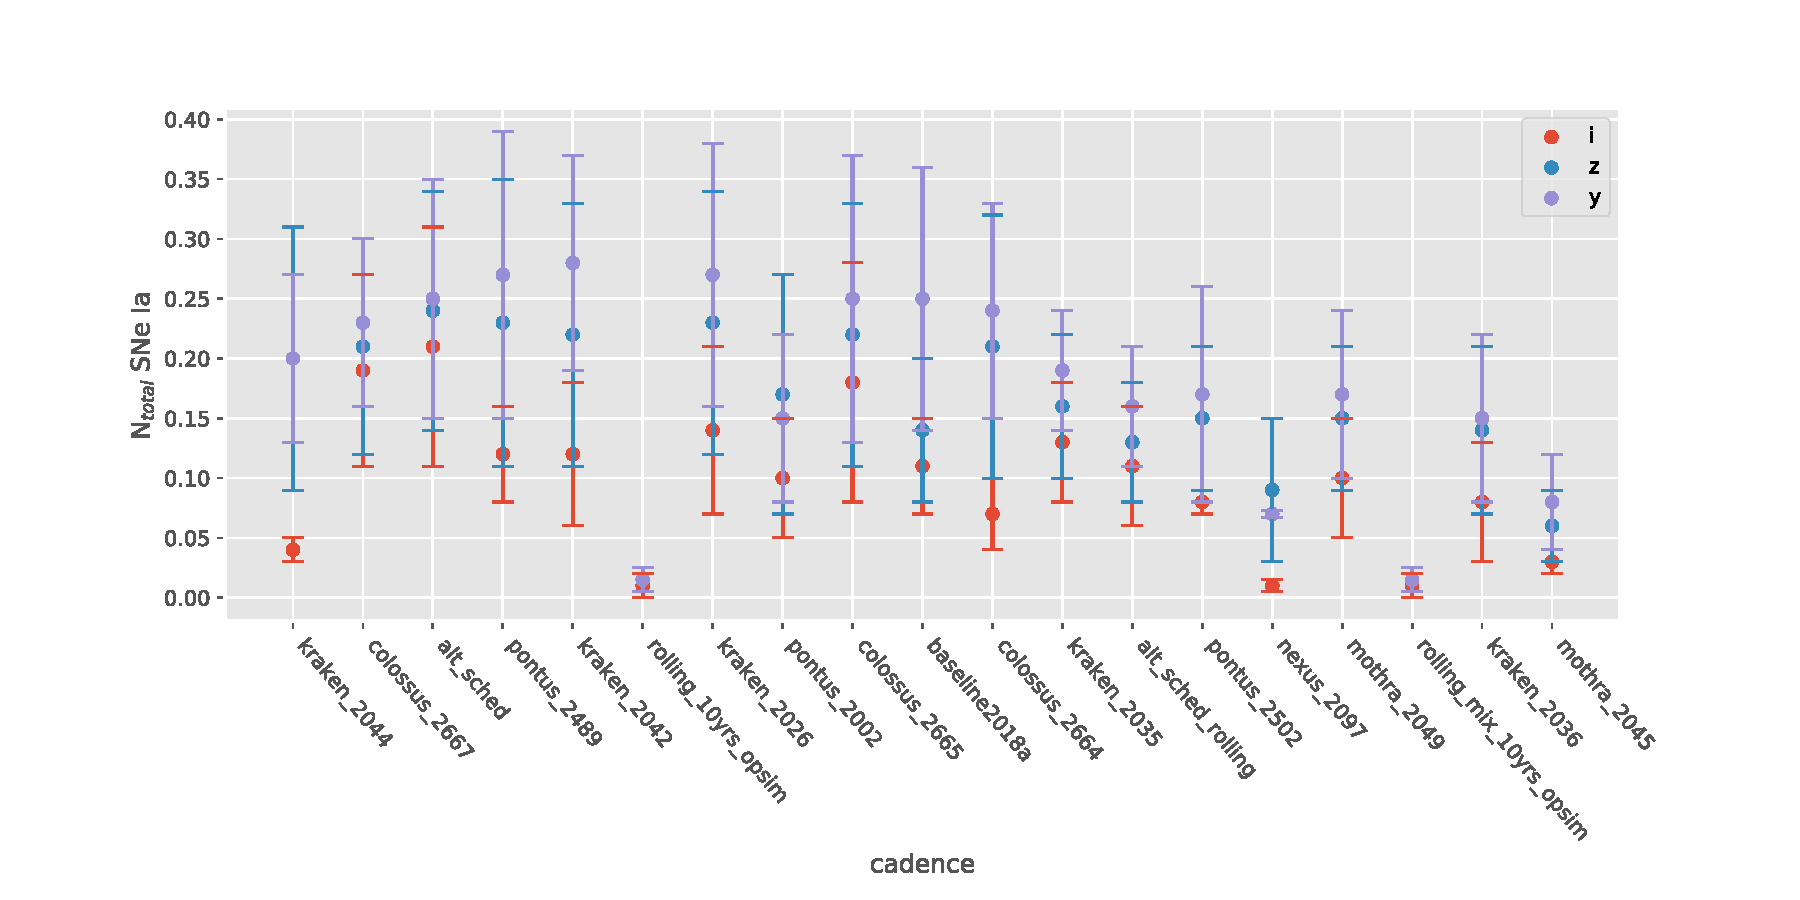
\includegraphics[scale=0.65]{figures/galaxy_lensing.pdf}\caption{The expected total number of strongly lensed SNe Ia arising from the multiply imaged galaxies in the Hubble Frontier Fields and Abell 1689 in function of the observing strategy. \todo{Tanja}{include new cadences and do same estimates for CC SNe*}}
\end{figure}

\FloatBarrier
\subsection{Lensed Quasars}
\textit{Contributors: TBD}
